\section{Selfish Mining}\label{sec:selfish-poc}

This section explores an example of experiment for an attack on the Bitcoin
network using \iblock{}. The attack is called \emph{selfish mining} and was
first described by \citeauthor{selfish-mining} in \citeyear{selfish-mining}
\cite{selfish-mining}.

\subsection{The Attack}\label{subsec:selfish-attack}

Bitcoin mining incentivizes block discovery by rewarding the miner with a block
subsidy and any transaction fees included within the block. This system aims to
maintain adherence to the protocol, encouraging honest mining behavior.
However, when a miner (or a group of colluding miners) controls over \(50\%\)
of the network's hash rate, network decentralization becomes compromised. Such
a miner can then select which transactions to confirm, enabling the potential
for double-spending, transaction censorship, and exclusive access to rewards,
effectively excluding others from mining gains.

\citeauthor{selfish-mining} in their work with the title
\citetitle{selfish-mining} proposed a strategy for a miner (or a pool of
colluding miners) to obtain a revenue larger than their fair share, allowing to
perform a successful attack even with a hash rate lower than \(50\%\).

The attack consists of a bad miner (the \emph{selfish miner}) that mines blocks
\emph{secretly} (i.e., without broadcasting them to the network). The miner
will let other miners mine on the public blockchain and, in the meantime, it
will mine on its own private chain. With \emph{enough} hash power, the miner
will be able to mine more blocks than the rest of the network, creating a fork
that, when published, will be selected by the network as the main chain as it
is longer than the public chain. Even with an hash power of less than \(50\%\),
the goddess Fortuna will sometimes come to the rescue. This way, the selfish
miner will be able to earn more rewards than the other miners that will lose
their revenue when the main branch is swapped to the selfish miner's fork. Also
note that the selfish miner will include, in his branch, even the transactions
that were included in the public branch, including those with the highest fees.

Moreover, it's worth noting that the selfish mining strategy has been
re-examined by its authors by developing a \emph{intermittent selfish miner}
which exploits the Bitcoin's difficulty adjustment mechanism to gain
more-than-fair revenues in absolute terms, not only in a relative sense
\cite{intermittent-selfish-mining}. Anyway this works only explores the
original selfish mining strategy.

\subsection{Selfish miner implementation}\label{subsec:selfish-impl}

The selfish miner implemented in \iblock{} diverges slightly from the
one proposed by \citeauthor{selfish-mining}. Their original approach is
structured as follows:
\begin{description}
	\item[Private Block Discovery] Upon discovering a new block, the
		selfish miner withholds it from the network, gaining a
		one-block lead over the public blockchain;
	\item[Trying its Luck] If the network discovers a block while the
		selfish miner holds a single-block lead, the miner publishes
		its private block, creating a fork and hoping that other miners
		choose to adopt his branch;
	\item[Extending the Lead] Upon finding additional blocks, the selfish miner
		refrains from broadcasting, extending the lead further;
	\item[Avoiding Catch-Up] When the lead reaches two blocks, and the
		network finds another block, the selfish miner publishes both
		withheld blocks, successfully outpacing the public chain.
	\item[Progressive Publishing] If the lead exceeds two blocks and the
		network discovers a new block, only the first unpublished block
		is broadcast. This preserves the two-block lead while starting
		to sequentially releasing the private chain.
\end{description}

There are some technical limitations on implementing the above strategy in the
actual implementation of \iblock{}:
\begin{description}
	\item[Memory Exhaustion] Indefinite growth of the private chain may
		lead to memory exhaustion, as \iblock{} must retains all blocks
		from the fork point onward;
	\item[Reward Calculation] To finalize rewards in \iblock{}, blocks must
		exceed the coinbase maturity parameter in confirmations.
		\iblock{}, in fact, consider the rewards as earned when the
		mined block reaches maturity. The selfish miner's chain,
		therefore, must remain shorter than the coinbase maturity
		parameter to ensure accurate reward computation;
	\item[All Nodes are Connected] Given \iblock{}'s fully connected
		network model, the selfish miner is unlikely to succeed if the
		private and public chains are identical in length. The other
		miners would generally confirm the honest chain before the
		selfish miner attempts to publicize its own, as they probably
		have already received the block from the other miners when the
		selfish miner realizes the public chain has caught up.
\end{description}

Consequently, in \iblock{}'s implementation, the selfish miner's private chain
is concealed until it reaches a maximum lead, lower than the coinbase maturity
parameter. Should the public chain catch up, the miner terminates the attack,
considering it a failure, and initiating a new chain from the updated public
blockchain.

The pseudocode for the implemented selfish miner can be seen in
Algorithm~\ref{alg:selfish-miner}. The algorithm is implemented by changing the
\code{BlockchainManager} application, while the \code{Miner} application is
still the same. The miner will work on the head of the selfish chain just
because the blockchain manager will trick the miner into thinking that the head
of the selfish chain is the legitimate main branch of the blockchain.

\begin{algorithm}
	\caption{\iblock{}'s selfish mining strategy}\label{alg:selfish-miner}
	\begin{algorithmic}[1]
		\Require \(N < COINBASE\_MATURITY\)\Comment{For correct reward
		computation}
		\Statex
		\Event{Init}
			\State \(maxSelfishChainLen \gets N\)\Comment{N taken
			from config}
			\State public chain \(\gets\) publicy known blocks
			\State selfish chain \(\gets\) publicy known blocks
			\State \(selfishChainLen \gets 0\)
			\State Mine at the head of the selfish chain
		\EndEvent
		\Statex
		\Event{I found a block}
			\State \(selfishChainLen \gets selfishChainLen + 1\)
			\State append new block to selfish chain
			\If{\(selfishChainLen =
			maxSelfishChainLen\)}\Comment{We won}
				\State Publish all of the selfish chain
				\State \(selfishChainLen \gets 0\)
			\EndIf
			\State Mine at the new head of the selfish chain
		\EndEvent
		\Statex
		\Event{Others found a block}
			\State append new block to public chain
			\State \(\Delta \gets\) length(selfish chain) -
			length(public chain)
			\If{\(\Delta < 0\)}\Comment{We didn't even find a
			single block}
				\State selfish chain \(\gets\) public chain
				\State \(selfishChainLen \gets 0\)
			\ElsIf{\(\Delta = 0\)}\Comment{They win}
				\State selfish chain \(\gets\) public chain
				\State \(selfishChainLen \gets 0\)
			\ElsIf{\(\Delta = 1\)}\Comment{Good guys are
			catching up\ldots}
				\State Publish all of the selfish
				chain\Comment{\ldots but we have already won!}
				\State \(selfishChainLen \gets 0\)
			\Else\Comment{\(\Delta \geq 2\) (increasing lead)}
				\State Do nothing
			\EndIf
			\State Mine at the head of the selfish chain
		\EndEvent
	\end{algorithmic}
\end{algorithm}


As this is a suboptimal implementation of the selfish miner, the attack
outcomes here may be slightly less favorable to the attacker than those
observed by \citeauthor{selfish-mining}. In their simulation, a selfish miner
controlling \(50\%\) of the network's hash rate could capture all rewards,
fully excluding other miners. While theoretically feasible, this outcome is
less likely in practice unless the selfish miner's private chain is allowed to
grow indefinitely --- a scenario with limited practical relevance since rewards
would remain inaccessible without eventual publication. In a real-world system,
some rewards would still be attainable by other miners, as the selfish miner
cannot always ensure winning every block publication race.

An example of this more practical approach of \iblock{} is, in fact, the
precence of the coinbase maturity parameter and the computation of mining
rewards that occur when the maturity is reached by the mined block. This
mirrors Bitcoin's protocol specification, where a \code{COINBASE\_MATURITY}
parameter (currently set to \(100\) blocks) sets the minimum confirmations
required before a miner can spend block rewards \cite[Chapter~``Coinbase
Transaction'']{learnmeabitcoin}. Thus, rewards are treated as secure and
definitive once maturity is reached, even if a longer chain later replaces the
current one. This approach, while more complex, is more realistic than
permitting the selfish miner to publish arbitrarily long chains, which would
erase even the earliest earned rewards --- the theoretical scenario considered
in \citeauthor{selfish-mining}'s analysis but less applicable in practice.

\subsection{The Model}\label{subsec:selfish-model}

For this analysis, two configurations were used. The first is named
``SelfishMining'' in file \texttt{simulations/pocs.ini} and has the following
characteristics:
\begin{itemize}
	\item 45 user nodes generating a transaction approximately every 15
		seconds;
	\item 4 \emph{honest} miners each contributing 20 TH/s to the total
		network's hash rate and creating transactions at the same rate;
	\item 1 \emph{selfish} miner node, with varying hash rate, also
		generating transactions at the same rate.
\end{itemize}

In total, the network consists of 50 nodes, producing about \(3.33\)
transactions per second globally.

The selfish miner is put in the configuration with six different level of
hash rate relative to the total network hash rate: \(10\%\), \(20\%\),
\(30\%\), \(40\%\), \(45\%\), and \(50\%\). Each of the six configuration has
been run 20 times with different random seeds and for 2 days of simulated time,
for a total of 120 simulations of 2 days each.

The other configuration is defined as ``HonestMining'' in the same file. It is
identical to the previous one, but the selfish miner is substituted with an
honest miner with the same varying hash rate of the selfish miner in the
previous configuration. Also this model has been run for a total of 120
simulations (20 for each hash rate level) of 2 days each.

\subsection{Result Analysis}\label{subsec:selfish-analysis}

The first part of the analysis examines the number of successful attacks
by the selfish miner at different hash rate levels. The results
are shown in Table~\ref{tab:selfish-attacks}. Naturally, higher hash rate
result in a higher number of successful attacks. The only exception appears at
the \(50\%\) hash rate level, where the selfish miner executed one fewer attack
than at the \(45\%\) level. This outcome reflects the miner's increased ability
to maintain a larger lead with a higher hash rate --- conducting fewer but more
impactful attacks.

\begin{table}[tbhp]
	\centering
	\begin{tabular}{|r|c|}
		\toprule
		Relative Hash Rate & Mean \# of Successfull Attacks \\
		\midrule
		\(10\%\) share (\(\approx8.888\) TH/s) & \(3.35\) \\[6pt]
		\(20\%\) share (\(20\) TH/s) & \(9.80\) \\[6pt]
		\(30\%\) share (\(\approx34.286\) TH/s) & \(14.55\) \\[6pt]
		\(40\%\) share (\(\approx53.333\) TH/s) & \(15.30\) \\[6pt]
		\(45\%\) share (\(\approx65.455\) TH/s) & \(17.05\) \\[6pt]
		\(50\%\) share (\(80\) TH/s) & \(16\) \\
		\bottomrule
	\end{tabular}
	\caption{Mean number of successful attacks performed by the selfish
	miner as its share of network's hash rate
	changes.}\label{tab:selfish-attacks}
\end{table}

The second part of this analysis focuses on the rewards earned by the single
miner with varying hash rate, operating either honestly or selfishly based on
configuration.  \figref{fig:selfish-reward} illustrates the results, with the
x-axis representing the miner's relative hash rate and the y-axis depicting the
miner's rewards as a percentage of total network rewards. Three lines are
displayed:
\begin{description}
	\item[Gray dashed line] shows the theoretical expected reward for
		honest mining with each hash rate level. This is, basically,
		the function \(y = x\) as the rewards are proportional to the
		hash rate;
	\item[Blue line] represents the average reward of the honest miner,
		with \(95\%\) confidence intervals, as obtained from the
		simulation;
	\item[Red line] represents the average reward of the selfish miner,
		with \(95\%\) confidence intervals, as obtained from the
		simulation.
\end{description}

\begin{figure}[tbhp]
	\centering
	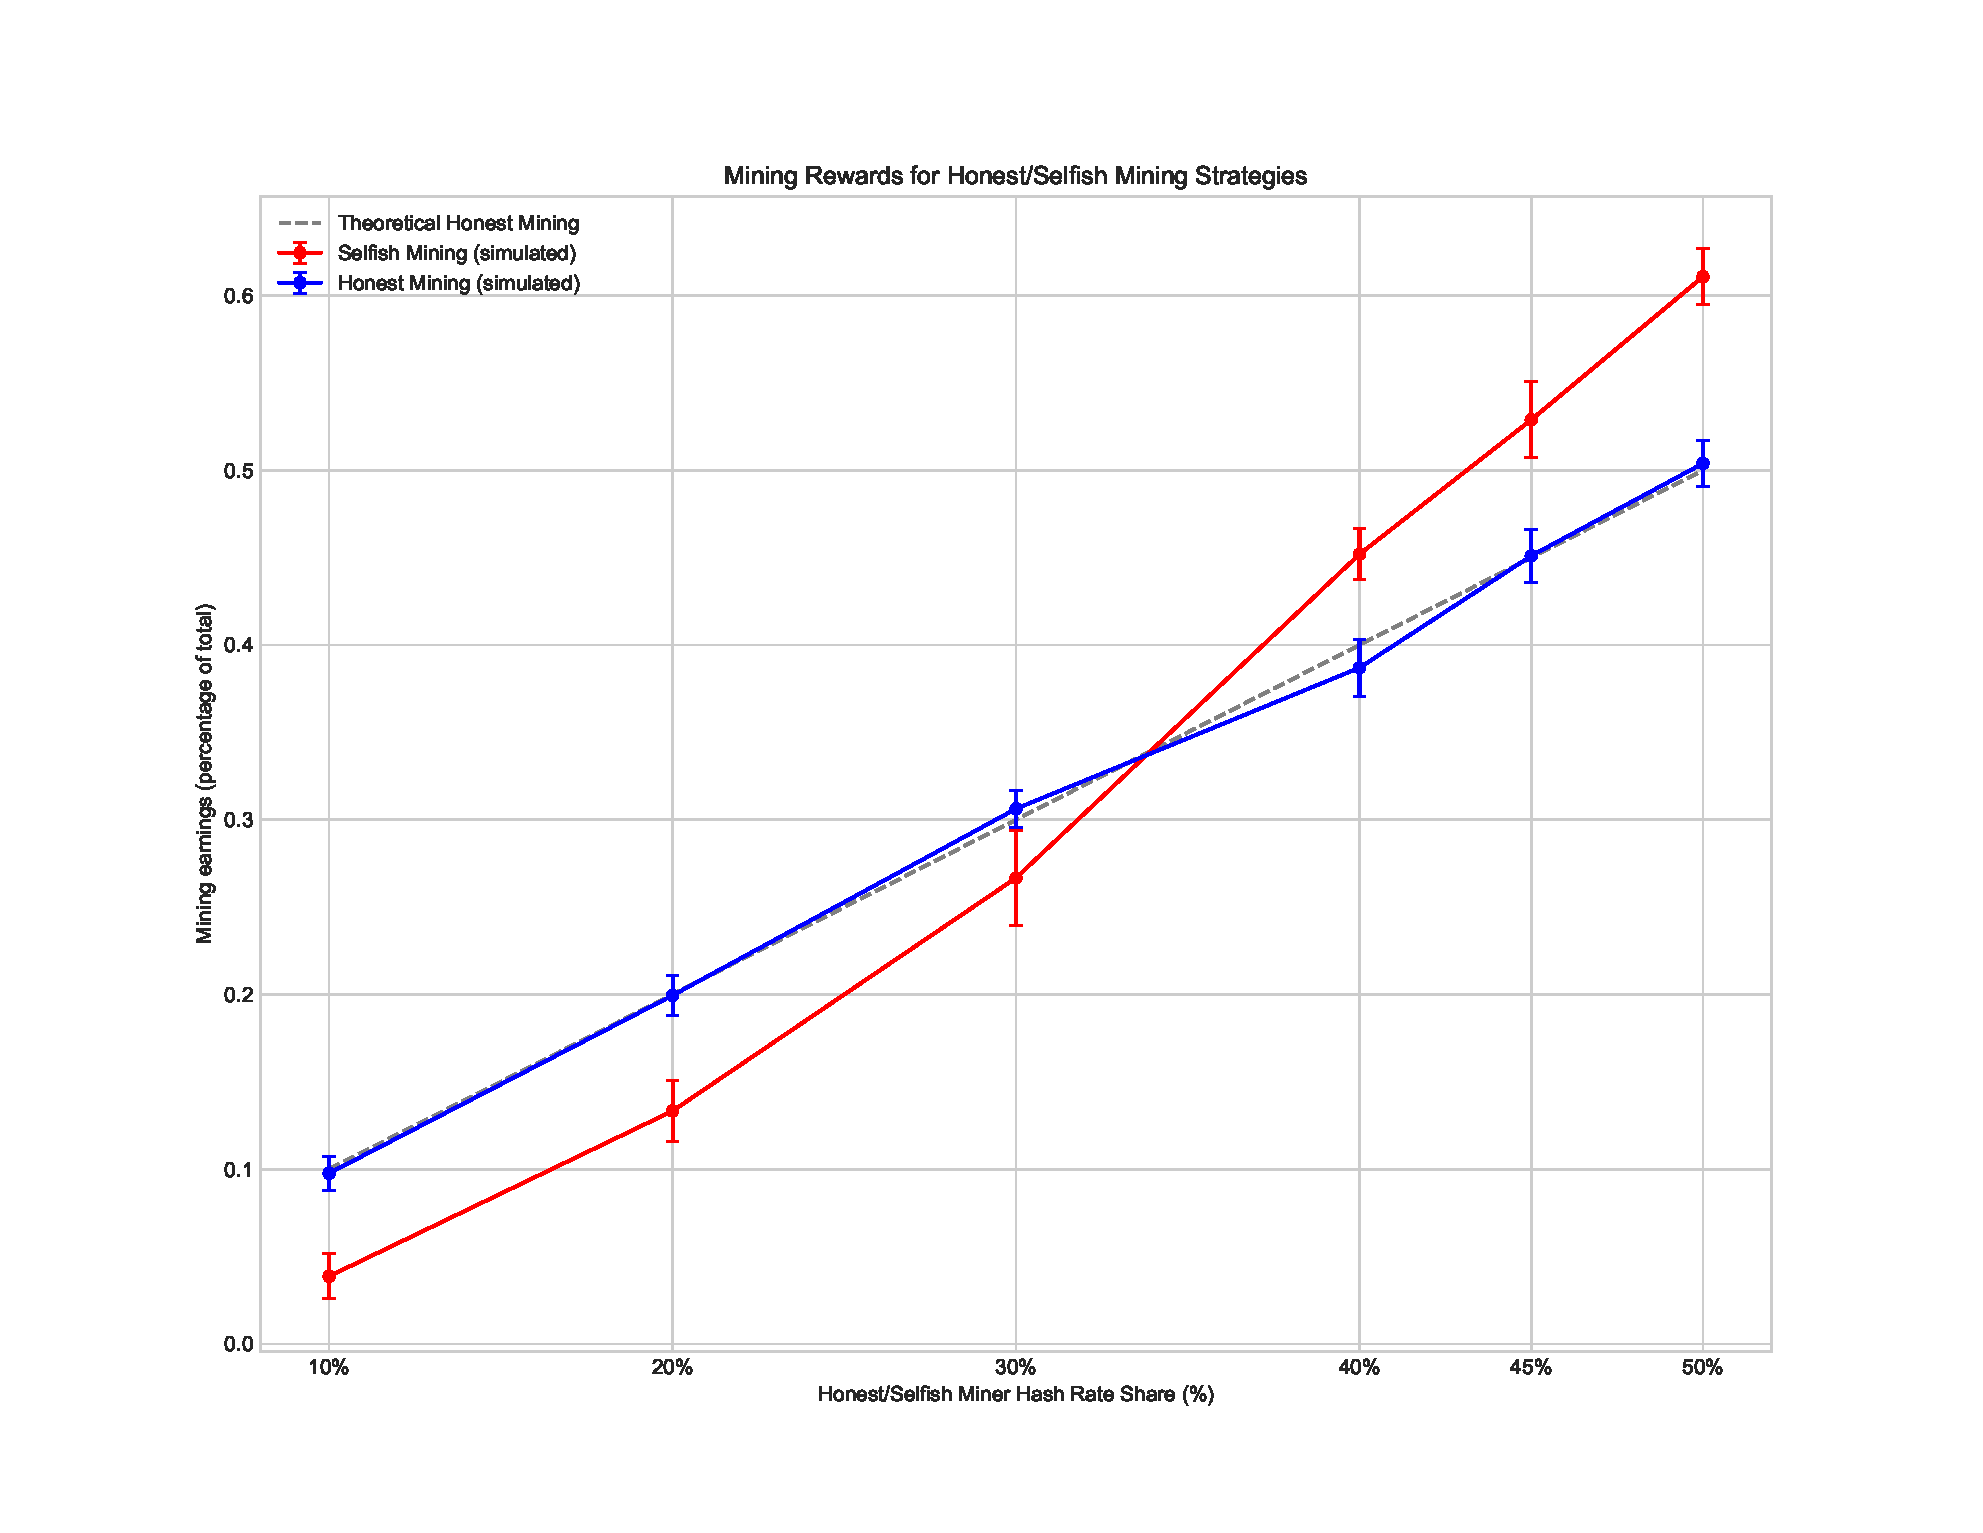
\includegraphics[width=\textwidth,trim={2.95cm 1.85cm 3.3cm
			2.5cm},clip]{selfish-mining-rewards}
	\caption{Relative mining revenues of the honest (blue) and selfish
	(red) miners across hash rate levels. \(95\%\) confidence intervals,
	based on 20 samples.}\label{fig:selfish-reward}
\end{figure}

The results indicate that the honest miner consistently receives expected
rewards, as the blue line's confidence intervals always overlap with the gray
dashed line, providing further validation of the accuracy of the \iblock{}
implementation.

For all hash rates below \(\frac{1}{3}\), the red line remains below the gray
dashed line (and also below the blue line), reflecting lower earnings for
selfish mining. However, once this threshold is surpassed, the selfish miner's
earnings exceed those of the honest miner. This result aligns with findings
reported by \citeauthor{selfish-mining}. The only difference, as anticipated
before, is that the results are a little worse than those obtained by
\citeauthor{selfish-mining}: with \(45\%\) of the hash rate, the selfish miner
should earn about the \(65\%\) of the total rewards (as claimed by
\citeauthor{selfish-mining}), while the results show a gain of ``only''
\(53\%\) on average; with \(50\%\), the selfish miner should earn all the
rewards, but it was able to gain only the \(61\%\) of the total rewards.

Nevertheless, the results are consistent with the expectations and the most
important result is confirmed: selfish mining becomes more profitable than
honest mining once the miner controls over \(\frac{1}{3}\) of the network's
hash rate. This align precisely with the outcomes obtained by
\citeauthor{selfish-mining} for the \(\gamma = 0\) case --- the scenario most
comparable to the \iblock{}'s setup, where a \emph{propagation factor}
\(\gamma\) of zero implies that honest miners avoid supporting the selfish
miner's chain when it lacks a lead. Remember, in fact, that \iblock{}'s
implementation of the selfish miner considers the attack failed when the public
chain reaches the height of the private chain. This provides further validation
of the correctness of the \iblock{} implementation.
